Most of the braille display products available in the market right now, such as those sold by HumanWare and RNIB, are based on piezoelectric bimorph benders or relay-lever mechanisms.  

The biomorph benders mechanism, shown in figure \ref{fig:piezo-bender} produces vibrations that move the pin up and down when placed in an electric field.
In relay-lever mechanisms, shown in figure \ref{fig:piezo-relay}, when voltage is supplied, the relay pushes the pin up. When the power is off, the weight of the lever mechanism moves the pin downwards to its original position \cite{hernandez_characterization_2009}.

\begin{figure}[ht] \centering
    \begin{subfigure}[b]{0.4\textwidth}\centering
        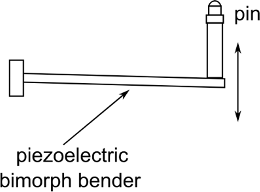
\includegraphics[height=3cm]{figures/piezo-bender-a.png}
        \caption{}
        \label{fig:piezo-bender}
    \end{subfigure}
    \begin{subfigure}[b]{0.4\textwidth}\centering
        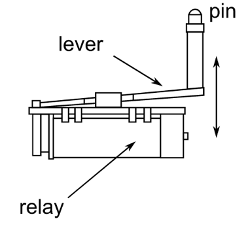
\includegraphics[height=3.5cm]{figures/piezo-bender-b.png}
        \caption{}
        \label{fig:piezo-relay}
    \end{subfigure}
\caption[Examples of existing Braille mechanisms]{Examples of existing Braille mechanisms: (a) piezoelectric bimorph bender and (b) relay-lever system \cite{hernandez_characterization_2009}.}
\label{fig:piezo-bender-schema}
\end{figure}

\todo[inline]{This moves from describing mechanism to condemning it. Requires information on what makes it burdensome, what is the cost and/or more concrete disadvantage why it's excluded.}
The main drawback of these two popular mechanisms is that benders and relay-lever systems are implemented as an additional burdensome module attached to the contact pins that may compromise integration capacity. According to [], a typical cell of biomorph piezoelectric braille display has a length of 40mm, and a commercial solution from Johnson Matthey has a length of 60mm for their 4×8 module, this means that a large space must be left between lines of cells in order for the biomorph bender to function properly. 
In consequence, Braille displays are not usually portable. Besides, the common cost for a single piezoelectric cell s about 100 US dollars to the end user, setting the price of even single line RBD well over 1000 dollars. The small size of the market also lead to a vicious cycle and limit the price from going down.
% Runyan, N., Blazie, D.: EAP actuators aid the quest for the ’Holy Braille’ of tactile displays. In: Y. Bar-Cohen (ed.) Electroactive Polymer Actuators and Devices, pp. 764,207–1 – 764,207–12. International Society for Optics and Photonics (2010). DOI 10.1117/12.847764 (reference for cost estimation)
% [1] is the reference for the burdensome module arguement,however, it doesn't provide any further detail and reference.

Another recently developed mechanism is piezoelectric ultrasonic motor \cite{hernandez_characterization_2009}.
The ultrasonic linear motor consists of a shaft, a mobile element or slider, and a piezoelectric ceramic disk as shown in figure \ref{fig:piezo-miniature}.
The key advantage of this design is the ultra-light weight of this miniature motor.
However, the need for several layers, as exemplified by figure \ref{fig:piezo-full-design}, does not befit the density required by a 2D tactile display.

\begin{figure}[ht] \centering
    \begin{subfigure}[b]{0.45\textwidth}\centering
        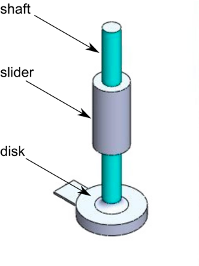
\includegraphics[height=5cm]{figures/piezo-miniature-a.png}
        \caption{}
        \label{fig:piezo-miniature-a}
    \end{subfigure}
    \begin{subfigure}[b]{0.45\textwidth}\centering
        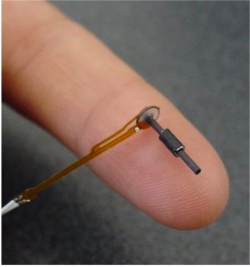
\includegraphics[height=5cm]{figures/piezo-miniature-b.png}
        \caption{}
        \label{fig:piezo-miniature-b}
    \end{subfigure}
\caption[Miniature piezoelectric linear motor]{Miniature piezoelectric linear motor: (a) conceptual design and (b) prototype.}
\label{fig:piezo-miniature}
\end{figure}

\todo[inline]{Add to caption: What is the value?}

\begin{figure}[ht]\centering
    \begin{subfigure}[b]{0.45\textwidth}\centering
        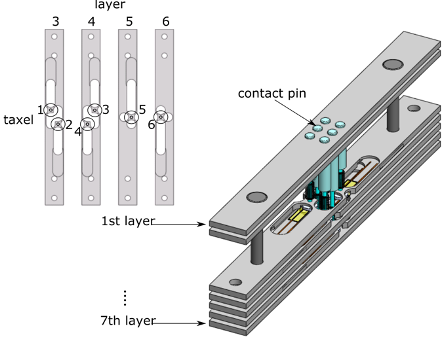
\includegraphics[height=5cm]{figures/piezo-full-design-a.png}
        \caption{}
    \end{subfigure}
    \begin{subfigure}[b]{0.45\textwidth}\centering
        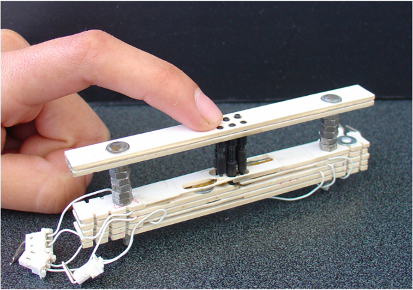
\includegraphics[height=4cm]{figures/piezo-full-design-b.png}
        \caption{}
    \end{subfigure}
\caption[Piezoelectric mechanism in-situ]{Piezoelectric mechanism in-situ. The requirement of several layers to create one cell makes it unviable for the density required by a 2D display.}
\label{fig:piezo-full-design}
\end{figure}